\documentclass{article}
\usepackage{amsmath}
\usepackage{amssymb}
\usepackage{./.sty/appendix}
\usepackage{graphicx}
\usepackage{multirow}
\usepackage{./.sty/titlesec}
\usepackage[dotinlabels]{./.sty/titletoc}
\usepackage[]{./.sty/mcode}
\usepackage{float}



\graphicspath{ {images/} }


\titlelabel{\thetitle.\quad}


\renewenvironment{abstract}
  {\small\quotation
  {\bfseries\noindent{\large\abstractname}\par\nobreak\smallskip}}
  {\endquotation}


\title{
	{A Numerical Solution to a Second Order Ordinary Differential Equation}\\
}


\author{
	Hunter, Marcus \\
	\and
	Tiger, Matthew \\
	\and
	Wigfield, Jacob \\
}


\begin{document}


\maketitle
\newpage


\tableofcontents
\newpage


\begin{section}{Introduction}
  The authors were tasked by the client with finding the solution to the following
family of differential equations
\[
  \begin{cases}
    -u''(x) + c u(x) = f(x) \\
    0 \leq x \leq 1 \\
    u(0) = \epsilon \\
    u(1) = \delta.
  \end{cases}
\]
Additionally, the client has also requested to be provided with a means of
plotting the solution once obtained.

Throughout this report, the above family of differential equations together with
the interval of definition and initial conditions will be represented by
$Lu = f$ where $L$ can be thought of as the differential operator for the above family.

Assumptions were placed on this family so that $c \in \mathbb{R}$ with $c > 0$
and $f \in C^k([0,1])$ for sufficiently large $k$ so that $f$ is relatively
well-behaved on the defined interval.

In this report we will detail the analytical solution to this family of
differential equations showing that the above problem is well-posed and
explain why this solution is not amenable to practical use. We therefore
provide a numerical scheme to approximate the solution to the family of
differential equations and examine the convergence, consistency and stability
of the numerical scheme. Using the solution provided by the numerical scheme,
we then explore the method for plotting the solution.

\end{section}


\begin{section}{Analytical Solution}
  The family of differential equations $Lu = f$ represents a second order linear
differential equation and therefore well-known techniques can be used to find
the solution $u(x)$.

The solution $u(x)$ is given by $u(x) = u_h(x) + u_p(x)$ where $u_h(x)$ is
the solution to the homogeneous equation $-u''(x) + c u(x) = 0$ and $u_p(x)$
is a particular solution of $-u''(x) + c u(x) = f(x)$.

To find the homogeneous solution, note that the characteristic equation of
this family of differential equations is given by $-m^2 + c = 0$, the roots of
which are $m_1 = \sqrt{c} = \omega $ and $m_2 = -\sqrt{c} = -\omega$. Note
that since $c > 0$, these roots are real and distinct suggesting that the
homogeneous solution is given by
\begin{align}\label{homogeneous_solution}
  u_h(x) = c_1 e^{\omega x} + c_2 e^{-\omega x}.
\end{align}

To find the particular solution, we assume the particular solution is of the
form $u_p(x) = \kappa(x) e^{\omega x}$ for some unknown function $\kappa(x)$.
Thus,
\[
u_p''(x) = \kappa''(x) e^{\omega x} + 2 \omega \kappa'(x) e^{\omega x} + \omega^2 \kappa(x) e^{\omega x}
\]
and substituting the above into the original differential equation $Lu = f$
with $u_p(x) = \kappa(x) e^{\omega x}$ we have
\begin{align}\label{particular_step_one}
  \kappa''(x) + 2\omega\kappa'(x) = -f(x)e^{-\omega x}.
\end{align}
Making the substitution $\lambda(x) = \kappa'(x)$ into \eqref{particular_step_one}
we can reduce the above second order linear differential equation into the
first order linear differential equation
\begin{align}\label{particular_step_two}
  \lambda'(x) + 2\omega\lambda(x) = -f(x)e^{-\omega x}.
\end{align}
The homogeneous solution to this first order differential equation is given by
$\lambda_h(x) = c_3 e^{-2\omega x}$ suggesting the particular solution to the
first order differential equation is of the form $\lambda_p(x) = \mu(x) e^{-2\omega x}$.

Repeating the same process as above, we see that
\[
\lambda_p'(x) = \mu'(x) e^{-2 \omega x} - 2 \omega\mu(x) e^{-2 \omega x}
\]
and substituting into \eqref{particular_step_two} with $\lambda_p(x) = \mu(x) e^{-2\omega x}$
we find that the first order linear differential equation becomes the separable first order differential
equation
\[
\mu'(x) = -f(x)e^{\omega x}.
\]
We readily see the solution to the above differential equation is given by
\[
\mu(x) = - \int_{0}^x f(r) e^{\omega r} dr.
\]
As $\kappa'(x) = \lambda_p(x) = \mu(x)e^{-2\omega x}$, we deduce that
\begin{align*}
  \kappa(x) = - \int_{0}^{x} e^{-2 \omega s} \left[ \int_{0}^s f(r) e^{\omega r} dr \right] ds
\end{align*}
and
\begin{align}\label{particular_solution}
  u_p(x) = \kappa(x)e^{\omega x} = -e^{\omega x} \int_{0}^{x} e^{-2 \omega s} \left[ \int_{0}^s f(r) e^{\omega r} dr \right] ds.
\end{align}
Combining the homogeneous solution \eqref{homogeneous_solution} and the particular
solution \eqref{particular_solution} we have that the general solution to
$Lu = f$ is given by
\begin{align}\label{general_analytical_solution}
  u(x) &= u_h(x) + u_p(x) \nonumber \\
  &= c_1 e^{\omega x} + c_2 e^{-\omega x} - e^{\omega x} \int_{0}^{x} e^{-2 \omega s} \left[ \int_{0}^s f(r) e^{\omega r} dr \right] ds.
\end{align}
Using the boundary values provided in $Lu=f$, the general solution is specified
by the system of linear equations
\begin{align*}
  u(0) &= c_1 + c_2 = \epsilon \\
  u(1) &= c_1 e^{\omega} + c_2 e^{-\omega} - e^{\omega} \int_{0}^{1} e^{-2 \omega s} \left[ \int_{0}^s f(r) e^{\omega r} dr \right] ds = \delta .
\end{align*}
The solution to this system in terms of the unknowns $c_1$ and $c_2$ is given
by
\begin{align*}
  c_1 = \frac{\epsilon e^{-\omega} - \delta - e^{\omega} \int_{0}^{1} e^{-2 \omega s} \left[ \int_{0}^s f(r) e^{\omega r} dr \right] ds}{e^{-\omega} - e^{\omega}}\\
  c_2 = \frac{-\epsilon e^{\omega} + \delta + e^{\omega} \int_{0}^{1} e^{-2 \omega s} \left[ \int_{0}^s f(r) e^{\omega r} dr \right] ds}{e^{-\omega} - e^{\omega}}.
\end{align*}

Using these constants in the general solution \eqref{general_analytical_solution}
gives us the unique analytical solution to the family of differential equation $Lu = f$.
Furthermore, we deduce that the problem is in fact well-posed.

From this solution, we must make the following additional assumption on this
problem: $f(x)$ must be integrable on the interval $[0, 1]$.

As the analytical solution depends on the symbolic integration of $f(x)$, we
will be unable to use this solution for functions $f(x)$ in which the
closed-form of the integral is not known.

\end{section}


\begin{section}{Numerical Scheme}\label{sec:scheme}
  As mentioned in the previous section, the analytical solution is not practical
to use for most functions $f(x)$. Thus, we present a numerical solution to
approximate the analytical solution for the problem $Lu = f$.

\begin{subsection}{Description}
  Our solution is derived from the method of finite differences. We define
  a finite set of points on the interval $[0, 1]$ called the grid $D_h$ where
  the parameter $h$ is the size of the grid where a smaller $h$ denotes a finer
  grid. For our purposes, we consider $h=1/N$ for positive $N$ and
  create the uniform grid
  \begin{align}\label{uniform_grid}
    D_h = \{x_n| x_n = hn \text{ for $0 \leq n \leq N$}\}.
  \end{align}

  Define on this grid the discretized solution to the problem $Lu = f$ as
  \begin{align}\label{discretized_solution}
    [u]_h = \{u(x_n)\}.
  \end{align}
  Similarly, define the discretized function of $f(x)$ as $f^{(h)} = \{f(x_n)\}$.
  We wish to create a scheme $L_h$ that computes an approximate solution
  $u^{(h)} = \left\{u_0^{(h)}, u_1^{(h)}, \dots, u_N^{(h)}\right\}$ to the problem
  $Lu = f$, i.e.\ a scheme such that $L_h u^{(h)} = f^{(h)}$.

  Finding an approximation to $u''(x)$ should suggest how to construct
  the scheme $L_h$.
  To find an approximation for $u''(x)$, we investigate the Taylor expansion
  of $u(x)$ centered at $h$ and $-h$. These expansions are given by
  \begin{align*}
    u(x + h) &= u(x) + h u'(x) + \frac{h^2 u ''(x)}{2} + \frac{h^3 u^{(3)}(x)}{3!} + \frac{h^4 u^{(4)}(\xi_1)}{4!} \\
    u(x - h) &= u(x) - h u'(x) + \frac{h^2 u ''(x)}{2} - \frac{h^3 u^{(3)}(x)}{3!} + \frac{h^4 u^{(4)}(\xi_2)}{4!}
  \end{align*}
  where $x \leq \xi_1 \leq x + h$ and $x - h \leq \xi_2 \leq x$.
  Adding these two expressions and solving for $u''(x)$ shows that
  \begin{align}\label{second_deriv}
    u''(x) = \frac{u(x + h) - 2u(x) + u(x-h)}{h^2} - \frac{h^2(u^{(4)}(\xi_1) + u^{(4)}(\xi_2))}{4!}.
  \end{align}
  This suggests that we should define our numerical scheme by replacing $u''(x)$
  in $Lu = f$ with the approximation
  \[
  u''(x) \approx \frac{u(x + h) - 2u(x) + u(x-h)}{h^2}.
  \]
  Therefore, we define the numerical scheme as
  \begin{align}\label{numerical_scheme}
    L_h u^{(h)} = f^{(h)} :=
    \begin{cases}
      \frac{-u_{n+1} + 2 u_n - u_{n-1}}{h^2} + c u_n = f_n & \text{for $n= 1, \dots, N - 1$} \\
      u_0 = \epsilon \\
      u_N = \delta
    \end{cases}.
  \end{align}
  For $n=1,\dots,N-1$, the scheme presents us with the recurrence relation
  \[
  -u_{n-1} + (2 + ch^2) u_n - u_{n+1} = h^2 f_n
  \]
  with initial conditions $u_0 = \epsilon$ and $u_N = \delta$. This recurrence
  relation is represented by the following system of equations
  \begin{align*}
    (2 + ch^2) u_1 - u_2 &= h^2f_1 + u_0 \\
    -u_1 + (2 + ch^2) u_2 - u_3 &= h^2f_2 \\
    -u_2 + (2 + ch^2) u_3 - u_4 &= h^2f_3 \\
    \vdots &  \\
    -u_{N-2} + (2 + ch^2) u_{N-1} &= h^2f_{N-1} + u_N.
  \end{align*}
  In matrix form, this system of equations becomes
  \begin{align}\label{matrix_system}
    \begin{bmatrix}
      2 + ch^2 & -1 & 0 & \hdots & 0\\
      -1 & 2 + ch^2 & -1 & \hdots & 0\\
      0 & -1 & 2 + ch^2 & \hdots & 0\\
      \vdots & \vdots & \vdots & \ddots & \vdots \\
      0 & 0 & 0 & \hdots & 2+ch^2 \\
    \end{bmatrix}
    \begin{bmatrix}
      u_1 \\
      u_2 \\
      u_3 \\
      \vdots \\
      u_{N-1}
    \end{bmatrix}
    =
    \begin{bmatrix}
      h^2 f_1 + u_0 \\
      h^2 f_2 \\
      h^2 f_3 \\
      \vdots \\
      h^2 f_{N-1} + u_{N}
    \end{bmatrix}
  \end{align}
  The solution to this system of equations paired with the initial conditions
  allows us to explicitly find $u^{(h)}$, our scheme's solution.

  In section \ref{sec:scheme_prop} we examine the convergence, consistency,
  and stability of this scheme in order to determine its usefulness in
  approximating the analytical solution to the problem $Lu = f$.
\end{subsection}

\begin{subsection}{Implementation}
  In order to efficiently use the numerical scheme just described we will need to
implement the scheme using computational software.

\subsubsection{Discretized Solution}
We have implemented the numerical scheme described above in MATLAB which can be
used by calling the m-function \texttt{numerical\_scheme.m}. We will now
describe the parameters necessary to call the function, how the function
computes the solution, and the results outputted by the function. Please refer
to appendix \ref{append_analytical} for the function definition in MATLAB.

This m-function requires the following parameters to compute the numerical solution:
\begin{itemize}
  \item \texttt{f} - MATLAB function that represents the function $f$ in the differential equation $Lu = f$.
  \item \texttt{c} - A real number that represents the constant $c$ in the differential equation $Lu = f$.
  \item \texttt{initials} - An array with two elements representing the initial conditions in the problem
    $Lu=f$. The first element of the array is $\epsilon$ and the second element of the array is $\delta$.
  \item \texttt{interval} - An array with two elements representing the endpoints of the interval of definition in
    the problem $Lu = f$.
  \item \texttt{subintervals} - An integer that represents the number of subintervals with which to construct
    the uniform nodes on the interval of definition. This corresponds to an
    $h$-value of $1/\texttt{subintervals}$ on the grid $D_h$.
\end{itemize}

Calling the function as follows
\[
  \texttt{numerical\_scheme(f, c, initials, interval, subintervals)}
\]
returns the array \texttt{[x, u]} where \texttt{x} is an array whose elements are
the nodes on the grid $D_h$ and \texttt{u} is an array whose elements are the
numerical solution obtained by the scheme $L_h u^{(h)} = f^{(h)}$ evaluated on the
nodes of the grid.

From these parameters, after verifying that $c$ is a positive real number,
the function creates and assigns to \texttt{x} the uniform
nodes equally spaced on the passed interval with width 1/\texttt{subintervals}. We then
construct the  coefficient matrix \texttt{A} and the right-hand side vector \texttt{b} of the equation
in \eqref{matrix_system}. Finally, we then assign to \texttt{u} the solution vector
which is given by \texttt{initials(1), A\textbackslash b, initials(2)}.

Using this function then allows us to compute the numerical solution to the problem
$Lu = f$.

\subsubsection{Plotting}
Now that we have an implementation to compute the numerical approximation to the
exact solution to the problem $Lu =f$, we would like to also have a way to plot
that solution.

In order to achieve that goal, we have implemented a function that performs
linear spline interpolation where the interpolants are the values of the computed
approximate solution using the numerical scheme $L_h u^{(h)} = f^{(h)}$.

The m-function \texttt{plot\_interpolation.m} takes as input the output from the
m-function \texttt{numerical\_scheme.m}, i.e.\ the nodes \texttt{x} and the
solution vector \texttt{u}. This produces a figure that plots the original
vector \texttt{u} and the linear splines that interpolate the elements of the
vector \texttt{u}.

As the number of nodes increases, the plot of the solution becomes smoother as
can be seen in Figure \ref{example_plot}.

\begin{figure}[h!]
  \begin{center}
    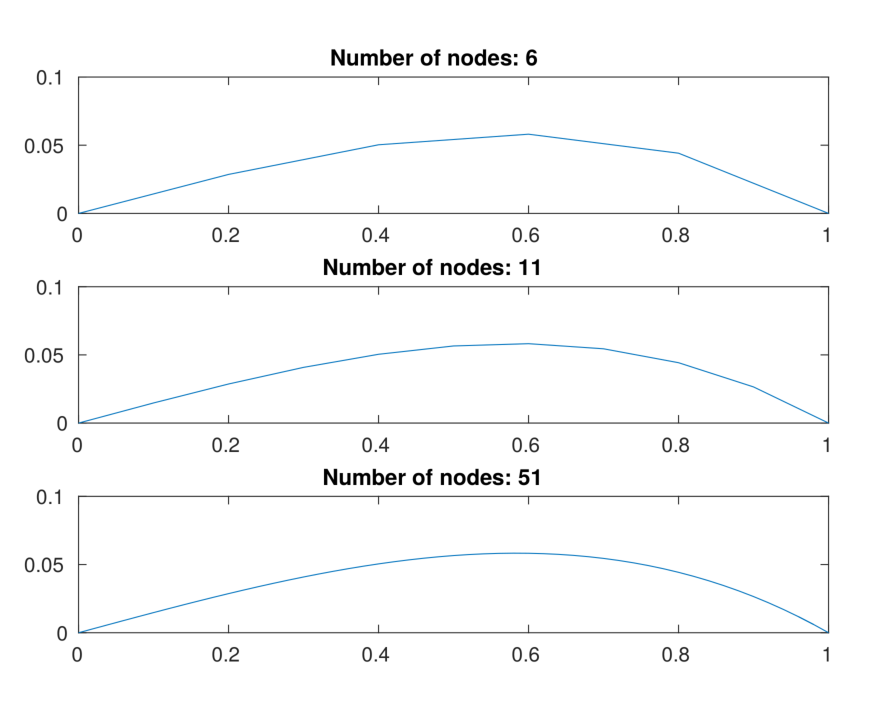
\includegraphics[scale=0.75]{example}
  \end{center}
  \caption{Plotted solution obtained from numerical scheme $L_h u^{(h)} = f^{(h)}$ for the problem $Lu = f$ with
    $f(x) = x$, $c =1$, and initial conditions $u(0) = 0$, $u(1) = 0$ for increasing number of nodes
    using the function \texttt{plot\_interpolation.m}.}\label{example_plot}
\end{figure}

We also have provided the m-function \texttt{linear\_interpolation.m} that evaluates
the solution obtained from the m-function \texttt{numerical\_scheme.m} for any $x$
on the interval of definition for the problem $Lu = f$. This is achieved
by evaluating the linear spline that interpolates the two nodes that contain
the point $x$ and returning that value.

The function definitions for \texttt{plot\_interpolation.m} and \texttt{linear\_interpolation.m}
can be found in Appendix \ref{append_plot}.
\end{subsection}

\end{section}


\begin{section}{Numerical Scheme Properties}\label{sec:scheme_prop}
  There are three main properties of the numerical scheme presented in section
\ref{sec:scheme} that are important to the validity of the numerical solution,
namely the convergence, consistency, and stability of the numerical scheme.
We will now investigate these properties in detail to determine how well
the numerical scheme approximates the analytical solution to our differential
equation.

\begin{subsection}{Convergence}
  The single most important property of the scheme presented in
\eqref{numerical_scheme} is its convergence to the analytical solution. We will
now rigorously define this notion of convergence.

But first, we must define the measure of the deviation between two solutions.
Let $U_h$ be the normed linear space of all functions defined on the grid $D_h$
as presented in \eqref{uniform_grid}. For $u^{h} \in U_h$, the equipped norm is
given as
\begin{align}\label{norm}
  ||u^{(h)}|| = \sup_n |u_n| = \max_n |u_n|.
\end{align}
With this definition, we can then precisely define the measure of deviation
between two solutions $a^{(h)}$ and $b^{(h)}$ as $||a^{(h)} - n^{(h)}||$.

Thus, we say that the solution $u^{(h)}$ given to us by the
scheme $L_h u^{(h)} = f^{(h)}$ \texttt{converges} to the discretized analytical
solution $[u]_h$ to the problem $Lu = f$ if
\begin{align}\label{convergence_def}
  ||[u]_h - u^{(h)}|| \to 0 \quad \text{as $h \to 0$}.
\end{align}

We now present strong numerical evidence that our scheme $L_h u^{(h)} = f^{(h)}$
converges to the discretized analytical solution to the problem $Lu = f$. The
program used to create the following tables can be found in appendix \ref{append_convergence}.

The following table shows the values of the computed norm $||[u]_h - u^{(h)}||$ for
increasingly smaller values of $h$ for $c=1$ on the interval $[0, 1]$ with the
initials conditions $u(0) = 1$ and $u(1) = 0.5$ with various definitions of
the function $f(x)$.

\begin{table}[h!]
  \centering
  \bgroup
  \def\arraystretch{1.5}
  \begin{tabular}{| l | c | c | c | c | c | c | c |}
    \hline
    $h$ & $x$ & $x^2$ & $x^3$ & $x^4$ & $x^5$ & $e^{0.5x}$ & $\sin(0.1 x)$\\
    \hline
    $10^{-1}$ & \texttt{0.2456e-4} & & & & & & \\
    $10^{-2}$ & & & & & & & \\
    $10^{-3}$ & & & & & & & \\
    $10^{-4}$ & & & & & & & \\
    \hline
  \end{tabular}
  \egroup
  \caption{Values of $||[u]_h - u^{(h)}||$ for various functions $f(x)$ with $c = 1$, $u(0) = 1$, and $u(1) = 0.5$.}
\end{table}

  % table for above
  %  0.026311866111212   0.149224341535297   0.249093262908154   0.313880742751841
  %  0.000264089528936   0.001504483908716   0.002496493222263   0.003175469244287
  %  0.000002630446940   0.000015056315862   0.000024978586145   0.000031769755671
  %  0.000000529416059   0.000000347104664   0.000000277642024   0.000000261196191

  % Columns 5 through 7

  %  0.365117561338677   0.077677335020362   0.059739448335529
  %  0.003682734158581   0.000780958308454   0.000602272840999
  %  0.000036840104460   0.000007822011283   0.000006011972430
  %  0.000000258153580   0.000000483720000   0.000000537327134


The above table suggests that the difference between the approximate solution
and the exact solution does tend toward zero as we refine the grid value $h$ and
that this happens regardless of the choice of $f(x)$.

A natural question would then be if the convergence is dependent upon the choice
of $c$. The following table shows the values of $||[u]_h - u^{h}||$ for various
increasing values of $c$ with $f(x) = e^{0.5x}$ and $u(0) = 1$, $u(1) = 0.5$.

\begin{table}[h!]
  \centering
  \bgroup
  \def\arraystretch{1.5}
  \begin{tabular}{| l | c | c | c | c | c | c | c |}
    \hline
    $h$ & $1$ & $17$ & $59$ & $119$ & $409$ & $1307$ & $14639$\\
    \hline
    $10^{-1}$ & & & & & & & \\
    $10^{-2}$ & & & & & & & \\
    $10^{-3}$ & & & & & & & \\
    $10^{-4}$ & & & & & & & \\
    \hline
  \end{tabular}
  \egroup
  \caption{Values of $||[u]_h - u^{(h)}||$ for various values of $c$ for the function $f(x) = e^{0.5x}$ with $u(0) = 1$ and $u(1) = 0.5$.}
\end{table}

The above table suggests that the convergence is not dependent on $c$ for $f(x) = e^{0.5x}$.

The last aspect of convergence to investigate is the impact of the initial conditions
on the scheme's convergence convergence. The following table shows the values of $||[u]_h - u^{h}||$ for various
initial conditions with $f(x) = e^{0.5x}$ and $c=1$.

\begin{table}[h!]
  \centering
  \bgroup
  \def\arraystretch{1.5}
  \begin{tabular}{| l | c | c | c | c | c |}
    \hline
    & $u(0) = 0$ & $u(0) = 0$ & $u(0) = -0.3$ & $u(0) = \phantom{-}1$ & $u(0) = -1$ \\
    $h$ &  $u(1) = 0$ & $u(1) = 0.01$ & $u(1) = \phantom{-}0.5$ & $u(1) = -1$ & $u(1) = -0.5$\\
    \hline
    $10^{-1}$ & & & & & \\
    $10^{-2}$ & & & & & \\
    $10^{-3}$ & & & & & \\
    $10^{-4}$ & & & & & \\
    \hline
  \end{tabular}
  \egroup
  \caption{Values of $||[u]_h - u^{(h)}||$ for various initial values for the function $f(x) = e^{0.5x}$ with $c=1$.}
\end{table}

Again, from the table we conclude that the approximate solution converges to the
exact solution regardless of the choice in initial conditions for the function
$f(x) = e^{0.5x}$.
\end{subsection}

\begin{subsection}{Consistency}
  The consistency of a numerical scheme is a measure of how well the solution
obtained by the scheme approximates the analytical solution as the grid
the scheme is defined on becomes more refined. Formally,
for a scheme $L_h u^{(h)} = f^{(h)}$ for the problem $Lu = f$, we say the
scheme is \textit{consistent} if
\begin{align}\label{consistency}
  ||L_h[u]_h - L_h u^{(h)}|| \to 0 \text{\ as $h \to 0$}
\end{align}
where $|| u^{(h)} ||$ is the norm defined on the normed linear space $U_h$ as
presented in \eqref{norm} in section \ref{convergence}.

Using the expression for the second
derivative in \eqref{second_deriv} and replacing it in our problem $Lu = f$, we
see that after some rearranging
\begin{align*}
  \frac{-u(x + h) + 2u(x) - u(x-h)}{h^2} + cu(x) = f(x) - \frac{h^2(u^{(4)}(\xi_1) + u^{(4)}(\xi_2))}{4!}.
\end{align*}
For the discretized analytical solution $[u]_h$ to our problem $Lu = f$ on the grid $D_h$,
this equation then becomes
\begin{align*}
  \frac{-u(x_{n+1}) + 2u(x_n) - u(x_{n-1})}{h^2} + cu(x_n) = f(x_n) - \frac{h^2(u^{(4)}(\xi_1) + u^{(4)}(\xi_2))}{4!}.
\end{align*}
From this equation we notice that the left side is precisely the evaluation
of our numerical scheme for the discretized analytical solution, i.e.
\begin{align}\label{discretized}
  L_h[u]_h = f_n - \frac{h^2(u^{(4)}(\xi_1) + u^{(4)}(\xi_2))}{4!}.
\end{align}
Combining the expression in \eqref{discretized} with the fact that
$L_hu^{(h)} = f_n$, we see that
\begin{align*}
  ||L_h[u]_h - L_hu^{(h)}||
  &= \left|\left| \left(f_n - \frac{h^2(u^{(4)}(\xi_1) + u^{(4)}(\xi_2))}{4!}\right) - f_n \right|\right| \\
  &= \left|\left| \frac{(u^{(4)}(\xi_1) + u^{(4)}(\xi_2))}{4!}\right|\right| h^2
\end{align*}

From the above equation it is clear that $||L_h[u]_h - L_hu^{(h)}|| \to 0$ as $h \to 0$.
Therefore, according to the definition in \eqref{consistency}, we see that
our scheme $L_h[u]_h = f^{(h)}$ is consistent.

If we make the assumption that the analytical solution's fourth derivative
is bounded, i.e. $|u^{(4)}(x)| \leq M$ for all $0 \leq x \leq 1$, then
\begin{align}\label{inequality}
  ||L_h[u]_h - L_hu^{(h)}||
  &= \left|\left| \frac{(u^{(4)}(\xi_1) + u^{(4)}(\xi_2))}{4!}\right|\right| h^2 \leq \frac{2M}{4!}h^2.
\end{align}
Moreover, from the inequality in \eqref{inequality}, we see that
\begin{align}\label{order}
  ||L_h[u]_h - L_hu^{(h)}|| \leq \frac{2M}{4!}h^2 = Ch^2
\end{align}
where the constant $C$ does not depend on $h$. In this case, we then say that
the scheme $L_h u^{(h)} = f^{(h)}$ has \textit{order of consistency} 2.

We thus conclude that as our scheme is consistent, it does in fact approximate
the analytical solution to the problem $Lu = f$ and approaches the analytical
solution as we refine the grid $D_h$.

\end{subsection}

\begin{subsection}{Stability}
\end{subsection}

\end{section}


% \begin{section}{Worked Example}
%   Specify a polynomial for f and set c and show how to implement solution and
then plot it.

% \end{section}

\newpage
\begin{appendices}
  \section{Analytical Solution Program}\label{append_analytical}
  The following is the m-function \texttt{analytical\_solution.m} for use in

  MATLAB to compute the analytical solution to the problem $Lu = f$. Returns
  a function handle to evaluate the analytical solution at any point on the
  interval [0, 1]. This function requires the symbolic toolbox in MATLAB.
  \lstinputlisting{../NumericalSolution/analytical_solution.m}

  \newpage
  \section{Numerical Scheme Program}\label{append_numerical}
  The following is the m-function \texttt{numerical\_scheme.m} for use in MATLAB
  to compute the numerical solution to the problem $Lu = f$.
  \lstinputlisting{../NumericalSolution/numerical_scheme.m}

  Note that the above m-function is dependent on the m-function
  \texttt{uniform\_nodes.m} and that it must be in MATLAB's path when using
  \texttt{numerical\_scheme.m}.
  \lstinputlisting{../NumericalSolution/uniform_nodes.m}

  \newpage
  \section{Numerical Scheme Convergence Program}\label{append_convergence}
  The following is the m-script \texttt{convergence.m} for use in MATLAB to
  produce a table displaying the convergence of the numerical scheme to the analytical
  solution.
  \lstinputlisting{../NumericalSolution/properties/convergence.m}

  This m-script is dependent upon the following m-function \texttt{convergence\_test.m}
  \lstinputlisting{../NumericalSolution/properties/convergence_test.m}

  \newpage
  \section{Numerical Scheme Stability Program}\label{append_stability}
  The following is the m-script \texttt{stability.m} for use in MATLAB to
  produce a table displaying the stability of the numerical scheme to the analytical
  solution.
  \lstinputlisting{../NumericalSolution/properties/stability.m}

  This m-script is dependent upon the following m-function \texttt{stability\_test.m}
  \lstinputlisting{../NumericalSolution/properties/stability_test.m}

\end{appendices}

\end{document}
